\documentclass[10pt,showpacs,preprintnumbers,footinbib,amsmath,amssymb,aps,prl,twocolumn,groupedaddress,superscriptaddress,showkeys]{revtex4-1}
\usepackage{graphicx}
\usepackage{dcolumn}
\usepackage{bm}
\usepackage[colorlinks=true,urlcolor=blue,citecolor=blue]{hyperref}
\usepackage{color}
\begin{document}
\title{Project 1}
\author{Parker Brue}
\affiliation{Department of Physics and Astronomy, Michigan State University, East Lansing, MI 48823}
\begin{abstract}
We present our Ferrari algorithm for solving linear equations. We wrote the one-dimensional Poisson equation, utilizing Dirichlet boundary conditions, as a linear set of equations and as a tridiagonal matrix. We compared a specialized algorithm for solving the tridiagonal matrix to an LU-decomposition of said matrix.  Our best algorithm, the specialized solver, runs as $4n$ FLOPS with $n$ the dimensionality of the matrix.
\end{abstract}
\maketitle

\section{Introduction}
As an introduction to the central ideas of the class, we studied the one-dimensional Poisson equation with Dirichlet boundary conditions. Namely, transforming the differential equation into a set of linear equations, and consequently, a matrix. We implemented a general algorithm, a specialized algorithm, and a LU-decomposition algorithm. In the course of this report, we introduce the theoretical model and the different algorithms  we developed, then discuss the results of the different methods. Important points of comparison lie with relative error and relative speed of the calculation due to FLOPS. 

\section{Theory}
	\subsection{Theoretical solution of the one dimensional Poisson equation}	
In general, the one dimensional Poisson equation reads as follows: \begin{equation} -u^{''}(x) = f(x)     \end{equation}  Through discretized approximation of {\it u}, we can solve for {\it f} using a set of linear equations: \begin{equation}
	f(x)=-\frac{v_{i+1}+u_{i-1}-2u_{i}}{h^{2}}      ;      i=1,...,n
	\end{equation}
Using Dirichlet boundary conditions, $u_{0}$  = $u_{n+1}$ = 0,  We can then rewrite this as a set of linear equations in the form of a tridiagonal matrix: \begin{equation}	
	\hat{A} \cdot \hat{u} = \hat{f}
	\end{equation}
Consequently, we can solve these linear equations through forward and backward substitution.

	\subsection{Specific Poisson equation}	
For our purposes of solving the Poisson equation, we assume a function \begin{equation}
	f(x)=100e^{-10x}
	\end{equation}
and a closed form solution with the Dirichlet boundary conditions:
	\begin{equation}
	u(x)=1-(1-e^{-10})x-e^{-10x}
	\end{equation}

	\subsection{Solving a Tridiagonal Matrix}
This is general tridiagonal matrix:
	\begin{center}
		$\begin{bmatrix}
			d_{1}& e_{1} & 0 & 0 \\
			e_{1} & d_{2} & e_{2} & 0 & \\
			0 & e_{2} & d_{3} & e_{i-n}   \\
			0 & 0 & e_{i-n} & d_{n} 
	
		\end{bmatrix}
		 \begin{bmatrix}
			u_{1} \\
			u_{2} \\
			u_{3} \\
			u_{n} 
		\end{bmatrix} =
		\begin{bmatrix}
			v_{1} \\
			v_{2} \\
			v_{3} \\
			v_{n}
		\end{bmatrix}$
		\end{center}

We can reduce this generalized matrix into an upper trianular matrix from forward and backward substitution. 
	
	\begin{equation}
	\tilde{f}_{i}=f_{i}-\frac{\tilde{f}_{i-1}e_{i-1}}{\tilde{d}_{i-1}} ; \tilde{d}_{i}=d_{i}-e^{2}_{i-1}/\tilde{d}_{i-1}
	\label{forward}
	\end{equation}
	
	\begin{equation}
	u_{i} = (\tilde{f}_{i}-e_{i}u{i+1})/\tilde{d}_{i}
	\label{backward}
	\end{equation}
where $d_{i}$ are the diagonal matrix elements and $e_{i}$ are the off diagonal matrix elements.

\begin{center}
		$\begin{bmatrix}
			d_{1}& e_{1} & 0 & 0 \\
			0 & \tilde{d}_{2} & e_{2} & 0 & \\
			0 & 0 & \tilde{d}_{3} & e_{n-1}   \\
			0 & 0 & 0 & \tilde{d}_{n} 
	
		\end{bmatrix}
		 \begin{bmatrix}
			u_{1} \\
			u_{2} \\
			u_{3} \\
			u_{n} 
		\end{bmatrix} =
		\begin{bmatrix}
			v_{1} \\
			v_{2} \\
			v_{3} \\
			v_{n}
		\end{bmatrix}$
		\end{center}
	


We were able to create another program that performed matrix mathematics to solve for the set of linear equations.  Taking a tridiagonal matrix, we can solve it using LU decomposition.
	
	\subsection{LU-decomposition}
	
	\begin{equation} \mathbf{A=LU} \end{equation}
$\mathbf{A}$, the matrix can be decomposed into the product of  $\mathbf{U}$, upper triangular matrix and $\mathbf{L}$, a lower triangular matrix
	\begin{equation} \mathbf{LUx=b} \end{equation}
	Which allows you to replace $\mathbf{A}$ and then use either triangular matrix to solve the problem.
	\begin{equation} \mathbf{Ly=b} \end{equation}
	\begin{equation} \mathbf{Ux=x} \end{equation}
\section{Algorithms}	

\section{Methods}
	\subsection{Relative error}

In order to properly test the effectiveness of our algorithm, we are measuring the closeness, or relative error of our analytic solution:

	\begin{equation}
	\epsilon_{i} = log_{10}(|\frac{v_{i}-u_{i}}{u_{i}}|)  ; i = 1,...,n
	\label{error}
	\end{equation}
$u_{i}$ is the analytic solution, and $v_{i}$ is the numerical solution.

\section{Results and discussions}

 We ran the program with the step sizes of n = 1, 2 , and 3, corresponding to a 10x10, 100x100, and 1000x1000 matrix. We also optimized our program through specialization. Diagonal matrix elements were set to 2 and off-diagonal elements were set to -1. FLOPS were reduced from 9 in the general case to 4 in the specialized case. The program was much more efficient, and faster as a consequence to the precalculation. 

 Analyzing step size, there is a clear difference from N=$10^{1}$ and N=$10^{2}$, while N=$10^{2}$ to N=$10^{3}$ does not seem to superficially change as much as is demonstrated in the graphs below.
 
%insert path specific for computer
\begin{figure}[!ht]
	\centering
	%\includegraphics[width=0.5\textwidth]{/Users/bruepark/Documents/GitHub/Physics480/project1/Report/out1.pdf}
	\includegraphics[width=0.5\textwidth]{/home/healthycheekums/Physics480/project1/Report/out1.pdf}
	\label{uvx}
	\caption{ n = 1. The x axis is the x values in the range [0,1] and the y axis is the resulting u values.}
\end{figure}

\begin{figure}[!ht]
	\centering
	%\includegraphics[width=0.5\textwidth]{/Users/bruepark/Documents/GitHub/Physics480/project1/Report/out2.pdf}
	\includegraphics[width=0.5\textwidth]{/home/healthycheekums/Physics480/project1/Report/out2.pdf}

	\label{uvx}
	\caption{n = 2. The x axis is the x values in the range [0,1] and the y axis is the resulting u values.}
\end{figure}

\begin{figure}[!ht]
	\centering
	%\includegraphics[width=0.5\textwidth]{/Users/bruepark/Documents/GitHub/Physics480/project1/Report/out3.pdf}
	\includegraphics[width=0.5\textwidth]{/home/healthycheekums/Physics480/project1/Report/out3.pdf}

	\label{uvx}
	\caption{n =3.  The x axis is the x values in the range [0,1] and the y axis is the resulting u values.}
\end{figure}

Further investigation shows that the overabundance of data points does give us the full curve, it also results in a much larger error, as shown in the table below. There seems to be a saddle point situated around N=$10^{2}$, wherein the calculation is optimized in regard to completeness of the graph and uncertainty from the numerical solution.

\begin{center}
	\begin{tabular}{cc}
		\hline \hline
			Step Size ($n$) &  Max Relative Error ($|\epsilon|$)\\
			\hline
			1 & 1.101\\
			2 & 3.079\\
			3 & 5.079\\
			4 & 7.079\\
			5 & 9.079\\
			6 & 11.50\\
			7 & 12.27\\
			\hline
			\label{errortable}
	\end{tabular}
\end{center}
	
	The above table shows us the absolute valued relative error results from varying step sizes of $N=10^{n}$ from 1 to 7. The step size error for n=7 seems to be the breaking point, the error starts to widely fluctuate. Therefore, the largest step size we would reccomend for an accurate result is n=6.  


	For further analysis, we included a timer in both the specialized program and the LU program, and compared the timing values for, for as large square matrices as either could reasonably calculate.

	\begin{center}
		\begin{tabular}{ccc}
			\hline \hline
			Column Size & Specialized Time (s) & LU Time (s)\\
			\hline
			10\textsuperscript{1} & 0.000430 & 0.00127\\
			10\textsuperscript{2} & 0.001830 &  0.09897\\
			10\textsuperscript{3} & 0.009720 & 31.4228\\
			10\textsuperscript{4} & 0.0750       &  --\\
			10\textsuperscript{5} & 0.7340  & --\\
			10\textsuperscript{6} & 7.820  & --\\
			10\textsuperscript{7} & 92.2239  & --\\
			\hline
			\label{timingtable}
		\end{tabular}
	\end{center}
	We found that specialized time was vastly more efficient over the LU time, as expected. We were unable to compute a LU matrix at $N=10^{4}$, initializing the program with this input would immediately sieze the program up. For the specialized solver, $N=10^{7}$ was the most reasonable limit, guessing at the size of the output file for $N=10^{7}$, ~400MB, we can assume that $N=10^{8}$ would not only take several hundred seconds to compute, but would result in a file size well over a GB, if not several. 	

\section{Conclusions}

\begin{thebibliography}{99}
\bibitem{miller2006} G.~A.~Miller, A.~K.~Opper, and E.~J.~Stephenson, Annu.~Rev.~Nucl.~Sci.~{\bf 56}, 253 (2006).
\end{thebibliography}

\end{document}